\subsection{Glyph: \glyph{Not}}
\label{sec:af:not}

The glyph \glyph{not} is used to denote that the \glyph{AN} linked as input cannot influence the target activity.

\begin{glyphDescription}
 \glyphSboTerm SBO:0000238 ! not.
 \glyphOrigin One \glyph{biological activity} (\sect{af:biologicalActivity}) or and a \glyph{logical arc} (\sect{af:logicArc}).
 \glyphTarget A \glyph{modulation arc} (~\sect{af:ANs}) other than \glyph{equivalence arc}.
 \glyphNode \glyph{Not} is represented by a circle carrying the word ``NOT'', with two connectors located at the opposite side for inputs and output.
 \end{glyphDescription}

\begin{figure}[H]
  \centering
  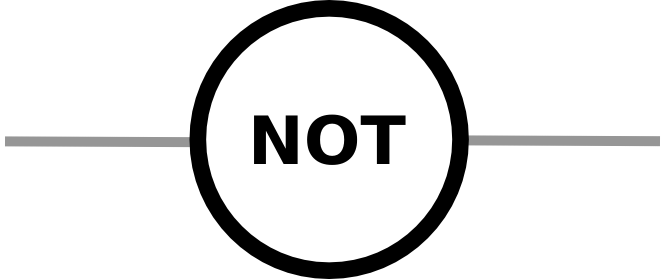
\includegraphics[scale = 0.5]{images/not}
  \caption{The \AF glyph for \glyph{not}.}
  \label{fig:af:not}
\end{figure}
